\chapter{Bewertung}
In diesem Kapitel wird das im vorherigen Kapitel beschriebene System beurteilt und mit dem vorhergehenden System verglichen.
Aufgrund der sich unterscheidenden Infrastrukturen der beiden Systeme, ist es nicht möglich einen direkten Vergleich durchzuführen.
Stattdessen müssen verschiedene Kennzahlen bezüglich der zu erfüllenden Anforderungen gefunden werden, um einen Vergleich zwischen den Kennzahlen des jeweiligen Systems durchzuführen.

\section{Abweichungen der Systeme}
Das in dieser Arbeit beschriebene System wurde besonders im Hinblick auf Ressourceneffizienz optimiert.
Somit gibt es auch starke Unterscheidungen zum alten System, welches lediglich ergebnisorientiert entworfen wurde und daher einen erhöhten Ressourcenverbrauch besitzt.

Um weniger Ressourcen zu verbrauchen wurde zum einen auch die Auswertung von Verkehrskamerabildern vereinfacht.
Statt der Verwendung eines neuronalen Netzes, welches einen sehr hohen Ressourcenbedarf mit sich zieht, wird nun ein weniger komplexer Background Subtraction Algorithmus verwendet.

Die Auswertung wird dadurch so stark vereinigt, dass sie sich auch auf die Clients auslagern lässt.
Das Backend kann also als einfacher Zwischenspeicher für Daten der Straßenverkehrszentrale Baden-Württemberg verwendet werden und ist somit auch für den Nutzen auf einem Shared Webhost optimiert.

Durch die Auslagerung der Auswertung auf die Clients ist jedoch auch nun der Großteil der Berechnung auf dem Client zu finden.
Es ist daher wichtig bestimmte Kenngrößen zu finden, um das eher client-lastige neue System mit dem server-lastigen Altsystem zu vergleichen.

\section{Kennzahlen}
Wichtige Kennzahlen für den Vergleich zwischen Neu- und Altsystem sollten vor allem die Anforderungen an das System widerspiegeln.
So ist es sinnvoll auch die während der Laufzeit benötigten Ressourcen zu messen, sowie die Genauigkeit des Systems zu bestimmen.
Während der Arbeit wurden folgende Kennzahlen zum Vergleich der Systeme bestimmt:
\begin{itemize}
\item{Arbeitsspeicher-Last des Systems}
\item{CPU-Last des jeweiligen Servers}
\item{Energieverbrauch des Clients}
\item{Genauigkeit des Systems}
\end{itemize}
Wobei die Arbeitsspeicher-Last des gesamten Systems jeweils am Client und am Server gemessen werden muss.

Diese Arbeit befasst sich aufgrund der Aufgabenstellung hauptsächlich mit der Optimierung der Arbeitsspeicher-Last.
Diese Ressource ist dabei auch eine der Ressourcen, welche kritisch für die Funktionalität des Systems sind.
Wenn das System an die Arbeitsspeichergrenze kommen würde, könnte dies bedeuten, dass die Applikation frühzeitig beendet wird oder erst gar nicht starten kann.
Wohingegen Energieverbrauch und CPU-Last meist nicht an konkrete Limitierungen gebunden sind.

\paragraph*{Nicht berücksichtigte Kennzahlen}

Da Sekundärspeicher in der heutigen Zeit relativ günstig ist und das System keinen hohen Gebrauch des Speichers macht, wurde dieser nicht für den Vergleich gemessen.
Ebenfalls wurde die Auswirkung von mehreren Clients auf das Ressourcen-Last nicht berücksichtigt, da das System in der Zielumgebung keine großen Nutzermengen unterstützen muss.


\newpage

\section{Datenerhebung}
*Wie sind Metriken messbar? Task-Manager, ...\newline
*Wie wurden Daten aufgenommen\newline
\paragraph*{CPU-Last}
\paragraph*{Arbeitsspeicher-Last}
\paragraph*{Energieverbrauch}
\paragraph*{Genauigkeit}
\newpage


\section{Auswertung}
\begin{figure}[ht]
   \centering
     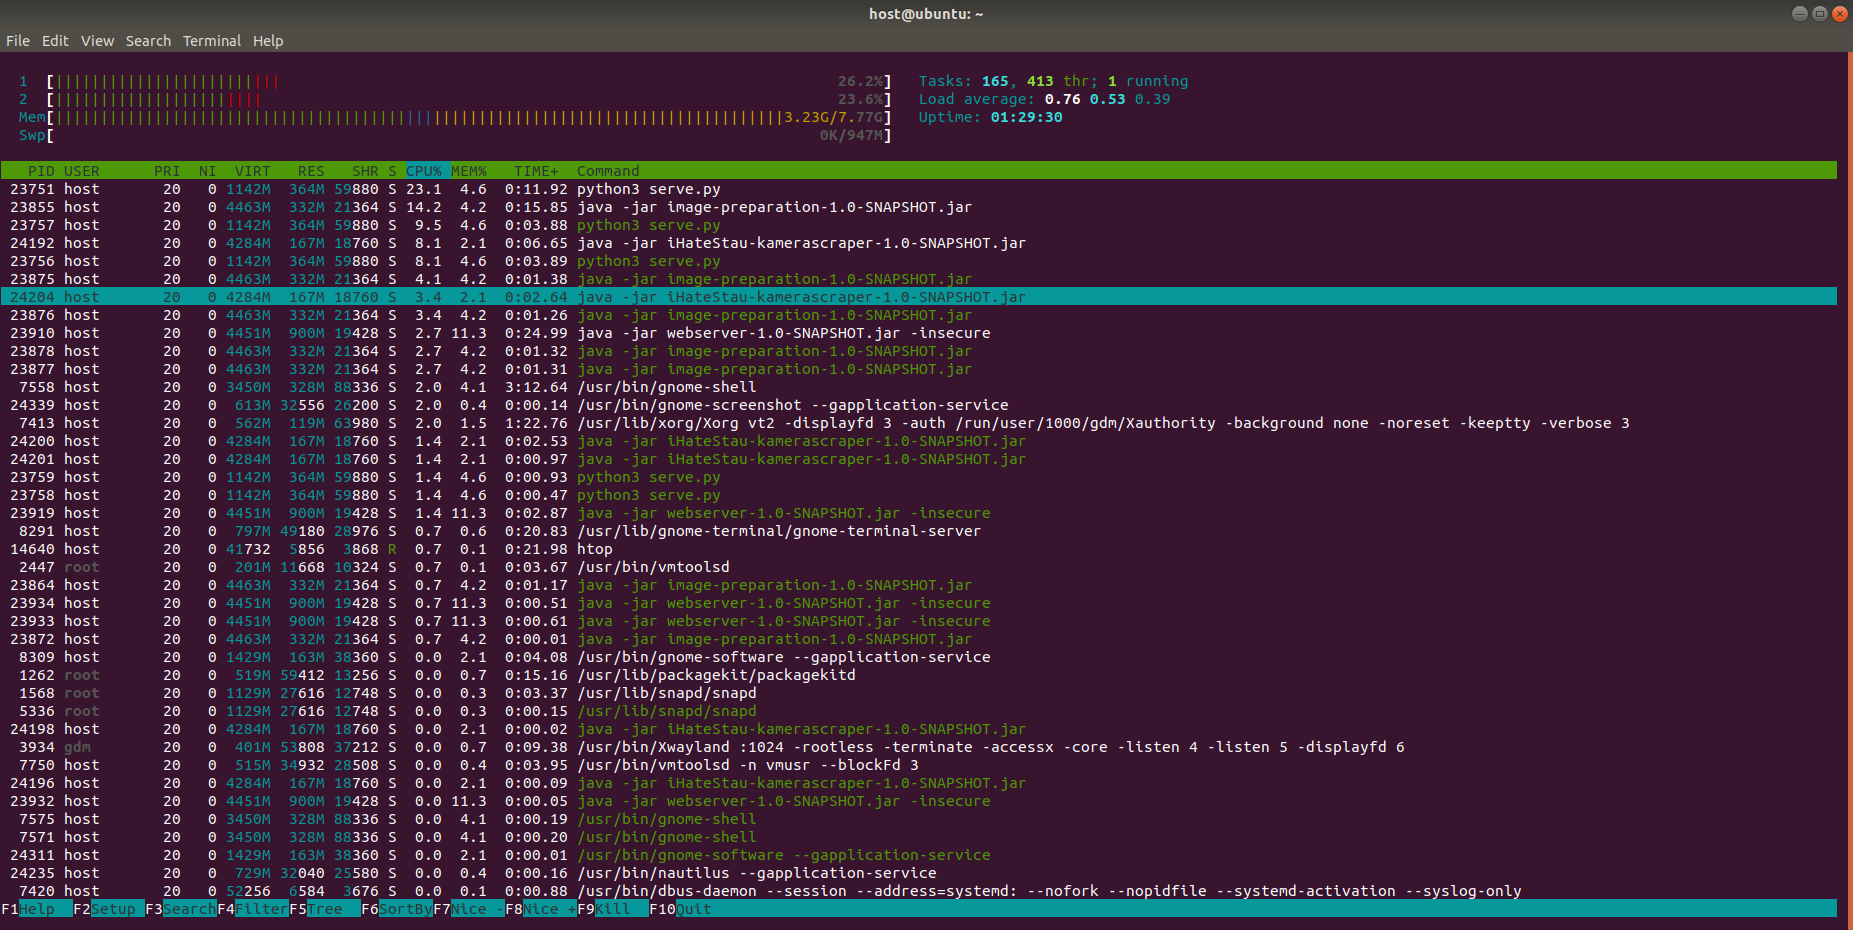
\includegraphics[width=15cm]{Bilder/server-ihatestau} \\
 \caption{Ressourcenverbrauch alter Server}
 \label{fig:ihatestau-res}
\end{figure}
\begin{figure}[ht]
   \centering
     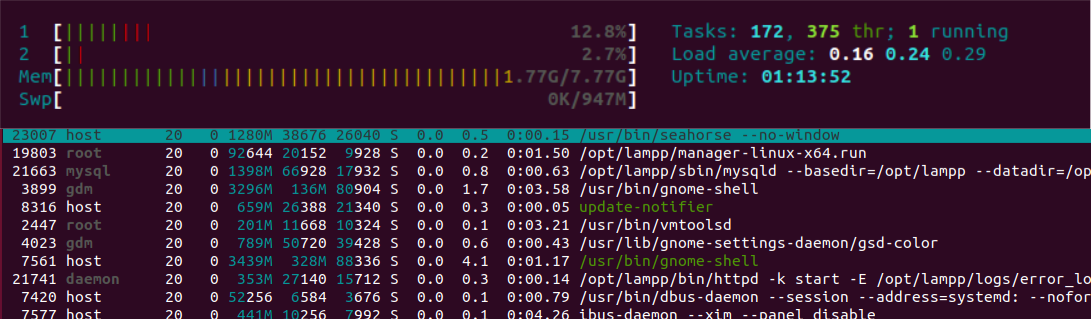
\includegraphics[width=15cm]{Bilder/server-new} \\
 \caption{Ressourcenverbrauch neuer Server}
 \label{fig:ihatestau-res}
\end{figure}
\begin{figure}[ht]
  \centering
	\begin{minipage}[b]{0.4\textwidth}
     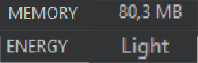
\includegraphics[width=\textwidth]{Bilder/res-app-old} \\
   \caption{Ressourcenverbrauch alter Client}
   \label{fig:res-app-old}
  \end{minipage}
	\hfill
	\begin{minipage}[b]{0.4\textwidth}
     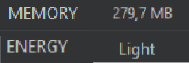
\includegraphics[width=\textwidth]{Bilder/res-app-new} \\
		\caption{Ressourcenverbrauch neuer Client}
		\label{fig:res-app-new}
	\end{minipage}
\end{figure}
\newpage

*Darstellung ggf. über Diagramme\newline
*Weniger genau aber auch weniger Ressourcen\newline
